\providecommand{\main}{..}
\documentclass[\main/master.tex]{subfiles}
\begin{document}
\chapter{Theoretical background}\label{chp:example-2}


\section{Torsional pendulum}
\subsection{Torsional pendulum}
A torsional Pendulum is an oscillator made of mass hung by a string from a fixed point alowing it to swing freelly. When the mass is displaced from the equilibrium angle, the pedulum has a liniar restoring torque, caused by the twisted string. The restoring torque rotates the mass back to the equilibrium position.


\begin{figure}[htbp]
	\centering
	\fbox{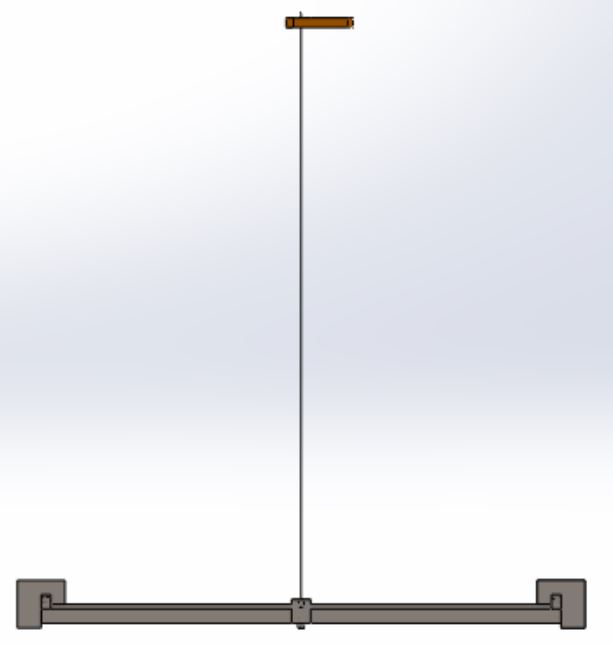
\includegraphics[scale=1.2]{\main/images/2 - theoretical background/torsion_pendulum.JPG}}
	\caption[Torsional pendulum]{A torsional pendulum}
	\label{fig:torsion_pendulum}
\end{figure}
\par\noindent

The pendulum can be assumed to be of two masses $m$ connected by a rigid, massless thin rod, with length of $2l$, and a pivot at distance $l$ from each side. When displaced from the equilibrium, there are two sources of torque; the displacing torque, and a liniar restoring torque at the opposite direction.
\begin{equation}
\tau = lFcos\theta -\kappa\theta    \label{eqn:Hooke_law}
\end{equation} 
At equilibrium, when balance stabilizes in a specific angle, the two sources of torque cancel each other out. 
With small equilibrium angle:
\begin{equation}
\tau = \kappa\theta = lF    \label{eqn:Hooke_law}
\end{equation}


\noindent
The string torsion coefficient $\kappa $ could be estimated, assuming homogeneousity of a circular string. Where $G$ is the material shear modulus, $J$ is the circular second moment of area ($Jzz$) and $h$ is the string length.
\begin{equation}
\kappa = \frac{GJ}{h} = \frac{G}{h} \frac{\pi D^4}{32}    \label{eqn:torsion_coefficient}
\end{equation}
Note, $\kappa$ could also be found empirically by finding  the  oscillations period.
 


\subsection{Simple harmonic oscillator}
The harmonic oscillator is a second order system that, when displaced, experiences a liniar restoring force proportional to the displacement from equilibrium. The torsional pendulum is an angular harmonic oscillator. It is equivalent to the liniar case, where instead of velosity and force, one has angular velosity and torque.
\par\noindent
If the restoring torque is the only torque acting then the oscillator is not driven or damped, one has a simple harmonic oscillator. The torque causes sinusoidal oscillations (simple harmonic motion) around the equilibrium angle.  
\begin{equation}
\tau = -\kappa\cdot\theta  = I\cdot\ddot{\theta}   \label{eqn:undamped_motion_equation}
\end{equation}
\begin{equation}
\theta(t) = \theta_{max}cos(\omega_0 t )    \label{eqn:undamped_motion_equation}
\end{equation}
\begin{equation}
\omega_0  = \frac{2\pi}{T} = \sqrt{\frac{\kappa}{I}}   \label{eqn:undamped_motion_equation}
\end{equation}
The moment of innertia of a rod with length $2l$ oscillating around a pivot is:
\begin{equation}
I = 2ml^2     \label{eqn:moment_innertia}
\end{equation}  
The natural resonant frequency $\omega_0$ and time period of oscillation $T$ are determined by the physical constants of the pendulum.


\subsection{Damped oscillator}
If the system is also having damping (friction) which is proportional to the velocity, the system is a damped oscillator.


\begin{equation}
\tau_{drag} = -b\cdot\dot{\theta}   \label{eqn:friction_torque}
\end{equation} 
\begin{equation}
\tau = -\kappa\cdot\theta - b\dot{\theta}  = I\cdot\ddot{\theta}   \label{eqn:damped_motion_equation}
\end{equation} 
\begin{equation}
\ddot{\theta} + 2\xi\omega_0\dot{\theta} + \omega_0^2\theta = 0   \label{eqn:damped_motion_equation}
\end{equation}
\noindent
The system damping ratio $\xi$ is the ratio between critical damping and the actual damping. The parameter determines the type of damping the system has, and the damping time of the system $\tau$. The damping ratio is a function of the damping coefficient $b$. The system could be either undamped, overdamped, critically damped or underdamped.
\begin{equation}
\theta(t) = Ae^{-\omega_0 t(\xi+\sqrt{\xi^2-1})} + Be^{-\omega_0 t(\xi-\sqrt{\xi^2-1})}    \label{eqn:damped_motion_equation}
\end{equation} 
\begin{equation}
\xi = \frac{b}{2\sqrt{I\kappa}} = \frac{actual}{critical}  \label{eqn:damped_motion_equation}
\end{equation}
\begin{equation}
\tau = \frac{1}{\xi\omega_0} = \frac{1}{\frac{b}{2\sqrt{I\kappa}}\sqrt{\frac{\kappa}{I}} }= \frac{2I}{b}  \label{eqn:damping_time}
\end{equation}
\begin{equation}
\theta(t) = Ae^{-\frac{t}{\tau}\cdot(1+\sqrt{1-\frac{1}{\xi^2}})} + Be^{-\frac{t}{\tau}\cdot(1-\sqrt{1-\frac{1}{\xi^2}})}    \label{eqn:damped_motion_equation}
\end{equation}
Undamped ($\xi = 0$); there is no friction and damping $b = 0$ leading to harmonic oscillations without decay.
\begin{equation}
\theta(t) = \theta_{max}cos(\omega_0 t )    \label{eqn:undamped_motion_equation}
\end{equation}
Overdamped ($\xi > 1$); due to high friction, the system cannot oscillate and it decays exponentialy to the equilibrium position.
\begin{equation}
\theta(t) = Ae^{-\frac{t}{\tau}\cdot(1+\sqrt{1-\frac{1}{\xi^2}})} + Be^{-\frac{t}{\tau}\cdot(1-\sqrt{1-\frac{1}{\xi^2}})}    \label{eqn:overdamped_motion_equation}
\end{equation}
Critically damped ($\xi = 1$); due to high friction, the system cannot oscillate and it decays exponentialy to the equilibrium position. For a fixed $I, \kappa$, choosing $b$ to be at the critical damping value would give the fastest return to the equilibrium position. Although there is overshoot this is often a desirable property.

\begin{equation}
\theta(t) = \theta_{max}\cdot e^{-\frac{t}{\tau}}     \label{eqn:underdamped_motion_equation}
\end{equation}
Underdamped ($\xi < 1$); amplitude decreases in time due to the friction while oscillating with a lower frequency due to the damping. 
\begin{equation}
\theta(t) = \theta_{max}\cdot e^{-\frac{t}{\tau}}cos(\sqrt{1-\xi^2}\omega_0 t ) =  \theta_{max}\cdot e^{-\frac{t}{\tau}}cos(\omega t )    \label{eqn:underdamped_motion_equation}
\end{equation}
When the damping coefficient is small enough, the frequency change is negligible.
\begin{equation}
\omega = \omega_0\sqrt{1-\xi^2}\approx\omega_0    \label{eqn:underdamped_frequency}
\end{equation}

\begin{figure}[htbp]
	\centering
	\fbox{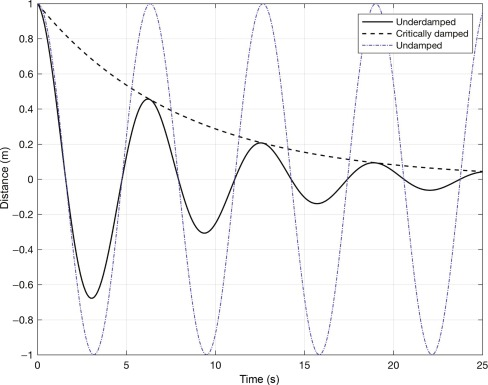
\includegraphics[scale=0.8]{\main/images/2 - theoretical background/damping.jpg}}
	\caption[Damped oscillators comparison]{Damped oscillators comparison; from sciencedirect \cite{underdamped-system}}
	\label{fig:damped_oscillators}
\end{figure}





\iffalse
https://ocw.mit.edu/courses/mathematics/18-03sc-differential-equations-fall-2011/unit-ii-second-order-constant-coefficient-linear-equations/damped-harmonic-oscillators/MIT18_03SCF11_s13_2text.pdf

https://www.sciencedirect.com/topics/engineering/underdamped-system#:~:text=When%20the%20damping%20ratio%20is%20between%200%20and%201%20(i.e.,is%20an%20exponential%20decay%20line.
\fi

\subsubsection{Driven oscillator}
If the damped oscillator system is further affected by an external time-dependent torque $\tau(t)$, the system is known as a driven oscillator.
\begin{equation}
\tau(t) -\kappa\cdot\theta - b\dot{\theta}  = I\cdot\ddot{\theta}   \label{eqn:driven_motion_equation}
\end{equation} 
\begin{equation}
\ddot{\theta} + 2\xi\omega_0\dot{\theta} + \omega_0^2\theta = \frac{\tau(t)}{I}   \label{eqn:damped_motion_equation}
\end{equation}






\section{Gravity measurement}

\subsection{Gravitational field}
Newton's law of universal gravitation states that every point mass attracts every other point mass in the universe.
\begin{equation}
\overrightarrow{F}(r) = \frac{GMm}{r^2}\hat{r}    \label{eqn:gravitation_force}
\end{equation} 
The force acts along the intersecting line, proportional to the product of the masses and inverse to the square of the distance between the centers. The inversity to the distance square means the force is very weak. For example the force between two cubes 1 kg each, 1 meter apart would be $\overrightarrow{F} = 6.67\cdot10^{-11} [N]$.
\par\noindent
The gravitational field of a mass is a vector field consisting at every point a vector pointing directly towards the particle. The magnitude of the field at every point is calculated by applying the universal law, the force per unit mass. 
\begin{equation}
\overrightarrow{G}(r) = \frac{\overrightarrow{F}(r)}{m} = \frac{GM}{r^2}\hat{r}    \label{eqn:gravitation_field}
\end{equation}
The field caused by a mass $M$ at a specific point is calculated by measuring the gravitational force. The gravitational force is caused by a known mass $M$ (a test mass). Test mass $M$ is much larger than each mass $m$, which ensures that there is a negligible influence on the behavior of $M$.  



\subsection{Cavendish experiment}
The Cavendish experiment, first performed in the 17th century, was the first experiment to measure the gravitational force between masses. The apparatus, which is constructed by a torsional pendulum is still used to accurately measure gravitational forces. Assuming no friction or other damping force (a simple harmonic oscillator) when a mass is interduced, there are two sources of torque in the system; torque by the mass gravitational force, and restoring torque caused by the wire torsion. Since gravity is a weak force, the torsional pendulum obeys Hooke’s law (due to small angles). At equilibrium, when balance has been stabilized at an angle $\theta$, these two torques are canceled out.
\begin{equation}
\tau = \kappa\theta = lF_g(r)    \label{eqn:gravitation_torque}
\end{equation}
\begin{equation}
\overline{\theta} = \frac{\tau}{\kappa} = \frac{\tau}{I\omega_0^2}    \label{eqn:theta average}
\end{equation}
The torsion string coefficient $\kappa$ could be estimated from the oscillations period. With accurate angle measurement, the gravitational force could be estimated.
 

\subsection{Gravity sensing}
The field at a specific point is the superposition of fields' point value. These fields are created by any mass in space. Measuring the gravitational field caused by a mass accurately, with a known test mass, the mass weight or distance could be estimated. In order to filter out the other gravitational fields caused by masses around, one measures the difference from a baseline state.
\par\noindent
Usually the measurement is with a frequency. The test mass moves in different frequencies, where not moving would be zero frequency. The masses around don't move, and are filtered out.
\par\noindent
The angle caused by the gravitational field is measured at each of those frequencies, measuring the energy spectral density $[\frac{rad}{\sqrt{Hz}}]$.
In the measurement system different noises have different frequencies. By integrating over long periods measurement noises are reduced. The signal to noise ratio (SNR) is the limiting factor for the sensitivity of a measuring system. In higher frequencies integration is faster, causing less noises and higher SNR.
The SNR dependency on frequency causes difficuties measuring gravitational fields at low frequencies.
\par\noindent
This is a significant challenge while designing gravimetric sensors.

\subsubsection{Shot noise limit}
A measuerment system can't measure a signal smaller than the system shot noise, which is a fundamental quantum physical phenomenon. Power fluctuations due to fluctuations in the number of photons. When measurement systems are optical, such as measuring angle displacement with a laser, the ground sensitivity and SNR that could be achieved are limited by the system shot noise.   
\begin{equation}
SNR = \frac{N}{\sqrt{N}} = \sqrt{N}    \label{eqn:shot_noise}
\end{equation}
While other system noises are higher than the shot noise limit, reducing noises and longer time integration would provide higher accuracy and better mesurement results. 

\section{Radiation pressure}
Radiation pressure is pressure on the surface due to momentum exchange with an electromagnetic field, including momentum of light. The light is at any wavelength which is absorbed, reflected, or emitted. The pressure causes force on the surface, although the force is usually insignificant.
  
\par\noindent
The radiation pressure force depends on the angle of surface compare to the electromagnetic field, as well as the surface intesity reflectance and absorbance, and the power of light hitting the surface $\Theta_i$ (radiant flux, measured in watts). There is coupling efficiency $\eta$ due to the light losses while passing through light transmitters (such as light guide or fiber), and size difference between the light beam size and the target size. In the equation below, the incident radiation pressure is calculated, when $\alpha$ is the field angle, compared to the surface area $A$, and $c$ the speed of light. As a first approximation one assumes, that the beam is focused tightly enough that variation over the surface is negligible. 
\begin{equation}
P_{incident} = \frac{\frac{\Theta_i}{A}cos^2(\alpha)}{c} = \frac{\eta\cdot \Theta_{source}\cdot cos^2(\alpha)}{{A\cdot c}} \label{eqn:radiation_pressure}
\end{equation}
The radiation pressure assuming light field direction perpendicular to surface and angle negligiblity is: 
\begin{equation}
P_{incident} = \frac{\eta\Theta_{source}}{{Ac}} \label{eqn:radiation_pressure_perpendicular}
\end{equation}

The radiation force assuming surface is a reflective material:
\begin{equation}
F = P_{total}\cdot A = (P_{incident}+P_{emitted})\cdot A = P_{incident}(1+R)A \label{eqn:radiation_force}
\end{equation}
\begin{equation}
F \approx 2P_{incident}A = \frac{2\eta\Theta_{source}}{{c}}\cdot \frac{A}{A} \label{eqn:radiation_force_reflective}
\end{equation}
\begin{equation}
F = \frac{2\eta\Theta_{source}}{{c}} \label{eqn:radiation_force_power}
\end{equation}

\section{Vacuum affects}

\subsection{Brownian motion}
Brownian motion is the pattern of random particles' fluctuations at fluid or gas, a random walk with no preferential direction of flow. This pattern happens at thermal equilibrium in a given temperature (on average there is no linear and angular momentum). 
\par\noindent
The average kinetic energy for a gas particle could be found from Maxwell-Boltzmann distribution of molecular speed, whereas the total Brownian motion kinetic energy is the sum over all gas particles.
\begin{equation}
f(v) = 4\pi(\frac{m}{2\pi kT})^{3/2}v^2exp(\frac{-mv^2}{2kT})     \label{eqn:Maxwell_Boltzmann}
\end{equation}  
\begin{equation}
<E_k>=<\frac{mv^2}{2}> = \int_{0}^{\infty}\frac{mv^2}{2}f(v)dv =  \frac{3kT}{2}    \label{eqn:avrage_kinetic}
\end{equation}
Gas pressure at a medium is propotional to the number density of particles.    
\begin{equation}
PV = Nk_BT  \label{eqn:ideal-gasses}
\end{equation}
\begin{equation}
E_k=N<E_k> =\frac{3}{2}Nk_BT = \frac{3}{2}PV    \label{eqn:total_kinetic}
\end{equation}

\noindent
The Brownian motion kinetic energy is proportional to the number of particles. Vacuum reduces the pressure and number of particles, which reduces the energy. There is energy coupling from the environment on the sides of the medium. Reducing the number of particles reduces the energy coupling.
\subsubsection{Brownian uncertainty}
The Brownian motion kinetic energy is proportional to the temperature. The noise of quantum uncertainty due to Brownian motion at a given temperature is: 
\begin{equation}
\frac{1}{2}\kappa (\delta\theta)^2= \frac{1}{2}KT  \label{eqn:radiation force}
\end{equation}
\begin{equation}
\delta\theta = \sqrt{\frac{KT}{\kappa}}\propto{T}  \label{eqn:radiation force}
\end{equation}

\subsection{Viscous friction}
The friction caused by gasses is viscous friction, which is velocity dependent. The velocity dependence is complicated. At very low speeds, gas resistance is approximately proportional to velocity: 

\begin{equation}
F_{drag} = -b\cdot v  \label{eqn:energy-mass-equivalence-relation}
\end{equation}

When Knudsen ratio is $0.01<k_n<0.5$, at a medium vacuum regime, the flow is called Knudsen flow. The molecules do not interact and move in straight lines between points. If chamber vaccum level is medium or higher, classical viscous friction of objects with gas particles inside the chamber could be negligible.

\subsubsection{Flow Characteristics}
Gas pressure at a medium is inverse to the mean free pass of each particle. A gas particle collides many times along it's way. It's mean free path is the average distance the particle could pass between two collisions with other particles. 


\begin{equation}
I = \frac{k_B\cdot T}{\sqrt{2}\cdot\pi\cdot p\cdot d_m^2}     \label{eqn:mean-free-pass}
\end{equation}
The Knudsen ratio which is used to characterize types of gas flow compare to the pipe diameter is derived from the above term.
\begin{equation}
K_n = \frac{I}{d}     \label{eqn:mean-free-pass}
\end{equation}

\subsection{Acoustic wave}
Acoustic waves are energy propagating through material, by adiabatic compression and decompression. The equation of one dimension acoustic wave, where the amplitude is acoustic pressure is:
\begin{equation}
P-P_0 = p = p_0cos(\omega t -\kappa x)       \label{eqn:acoustic_pressure}
\end{equation}
\begin{equation}
I = pV      \label{eqn:acoustic_intensity}
\end{equation} 
The power carried by acoustic waves $[\frac{W}{m^2}]$, known as acoustic intensity, depends on the material acoustic pressure and particle velosity. When the material pressure is reduced, the acoustic pressure is lower and less power is carried.

\subsection{Vacuum quality}
\subsubsection{Leak rate}
At any gas system, some gas would slowly leak over time and increase the pressure if not pumped out. The leak rate $Q_L$ is not a function of time but rather of volume, and resuls in a sustained increase of pressure P over time.
\begin{equation}
Q_L = \frac{\Delta P\cdot V}{\Delta t}  \label{eqn:energy-mass-equivalence-relation}
\end{equation}
The leak rate could prevant the system from reaching initial low pressure, since at some point the leakage would be equal to the pumping rate.
\par\noindent
There is also a diffusion rate of gas molecules, such as helium, which is insignifant when pressure is above $10^{-9}$ [Torr] (vacuum lower than high vacuum). 

\subsubsection{Outgassing}
At low pressures, there are more gas molecules adsorbed on the chamber surface than floating in the chamber. When pressure is below vapour pressure theres a desorption of gas molecules (primarily water) from the material.
\par\noindent
Outgassing is the desorption rate $Q_{des}$ which over time increases the pressure. The desorption rate depends on the surface area and the desorption density $q_{des}$ which is area specific. 
\begin{equation}
Q_{des} = q_{des}\cdot A\cdot\frac{t_0}{t}  \label{eqn:energy-mass-equivalence-relation}
\end{equation}
The desorption rate produces a gas yield that declines over time. It could be assumed that after a given time $t>t_0$ the increase is liniar over time, typicaly $t_0$ assumed to be one hour.
\par\noindent
Outgassing is minimized by selection of low vapor pressure materials such as stainless steel and glass. Since water is a significant source of outgassing, it is usually minimized by baking the chamber at high temperatures while the pump is running.


\section{Proportional–integral–derivative (PID) controller}
Proportional–integral–derivative controller (PID controller) is a feedback based control system. The control loop is used for time continuous control of a process, so the process output (measured process variable) would be close to a defined set point.
\par\noindent
PID controller continuously calculates error value, which is the distance of the measured process variable from the defined set point. The feedback applies an external correction to the process, called control variable. The control variable is based on a gain to the error of proportional $P$, integral $I$ and derivative $D$. Proper tuning of a PID enables an accurate automated correction to a controled process. The PID concept is used widely in applications requiring accurate automated control.

\par\noindent
The error and it's integral and derivate are calculated continuously. The control has three tuning parameters; $K_P, K_I, K_D$, the feed back correction is modulated by the tuning parameters' value. Each parameter is assigned to a gain (P-I-D). The response (control variable) is a weighted sum of the control terms. Over time the controller attempts to minimize the error $e(t)$ by adjusting the control variable $u(t)$, which is the PID output.
\par\noindent
\begin{figure}[htbp]
	\centering
	\fbox{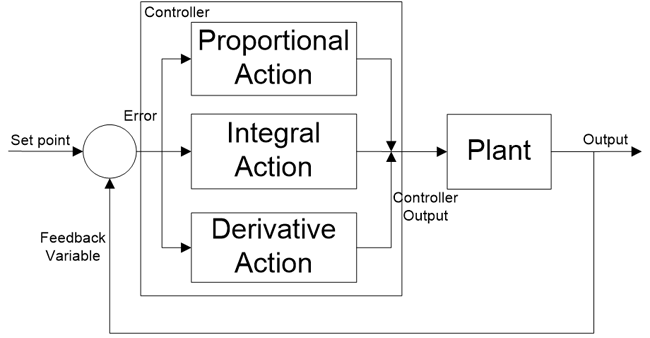
\includegraphics[scale=0.4]{\main/images/2 - theoretical background/PID.png}}
	\caption[PID controller block diagram]{PID controller block diagram; from circuitdigest \cite{PID-diagram}}
	\label{fig:PID_scheme}
\end{figure}
\begin{equation}
u(t) = K_Pe(t)+K_I\int_{0}^{t}e(t)+K_D\frac{de(t)}{dt}   \label{eqn:PID_eq}
\end{equation}

\noindent
P is proportional to the current error value $e(t)$. When error is large and positive, proportional output would be proportionately large and positive.
\par\noindent
I is proportional to past error value's integration. The response of the cumulative value could eliminate residual errors, such as signal offset.
\par\noindent
D is proportional to error current change rate, by calculating the derivative. The response of the change rate could eliminate more rapid changes.
\par\noindent
The optimal control function is achieved by balancing the responses. The tuning constants depend on the characteristics of the specific process. The response must be tuned for each control application.  


\end{document}







